\documentclass[../main.tex]{subfiles}
\graphicspath{{\subfix{../images/}}, {\subfix{../diagrams/}}}

\begin{document}

    \chapter{Architettura Cloud}
    
        Per poter sfruttare il processo \emph{DevOps} descritto in precedenza, si necessita della creazione di una infrastruttura cloud che possa ospitare e gestire gli strumenti, i flussi, i dati e le utenze necessarie al processo stesso. In questo capitolo verrà descritta l'architettura in modo più specifico, come sono state definite le risorse e configurati gli strumenti utilizzati.
	
	    \section{Introduzione e Definizione}
	    
	        Ogni strumento introdotto nel processo, necessita di un set di risorse fornite dal \emph{cloud provider} in misura tale da riuscire a gestire le sue operazioni efficacemente ma al contempo ridurre i costi dove possibile. Nel nostro caso, ogni strumento necessita obbligatoriamente di una \textbf{istanza server} dove essere \emph{hostato} singolarmente, ovvero ognuno ha una sua macchina dedicata e non condivide ambiente e dati con gli altri, un \textbf{metodo di accesso} ad esso in modo sicuro ed affidabile (possibilmente HTTPS) e la possibilità di non esporre su internet tali istanze così da ridurre al minimo possibilità di attacchi informatici a causa di vulnerabilità non corrette.\\*
	        
	        A seguito della analisi dei requisiti necessari, sono emerse le seguenti necessità a livello di risorse cloud da utilizzare:
	        \begin{itemize}
	            \item Le risorse devono essere raccolte in una rete virtuale \textbf{AWS VPC} per interconnetterle senza sforzi ulteriori;
	            \item Ogni istanza sarà definita con una macchina virtuale (VM) su \textbf{AWS EC2};
	            \item Per accedere allo strumento installato sull'istanza si dovrà agganciare un \textbf{Load Balancer} (di tipo variabile in base alle richieste), sui cui verrà installato il certificato per l'utilizzo in \textbf{HTTPS} e che fornirà \emph{TLS Termination} semplificando il setup della rete dietro di esso;
	            \item Se lo strumento necessita di un database relazionale (Phabricator, SonarQube) verrà creata una istanza dell'engine necessario utilizzando \textbf{AWS RDS} nella stessa rete creata;
	            \item Per permettere l'accesso sicuro e controllato alle risorse in cloud, si utilizzerà una istanza di \textbf{AWS Client VPN} con relativi certificati da rilasciare ai client abilitati.
	        \end{itemize}
	
	        Seguendo queste linee guida si è così definita una architettura cloud complessiva che potesse rispondere con successo alle esigenze del processo.
	
    	\section{Diagramma Architetturale}
    	
    	    \begin{figure}[H]
    			\centering
    			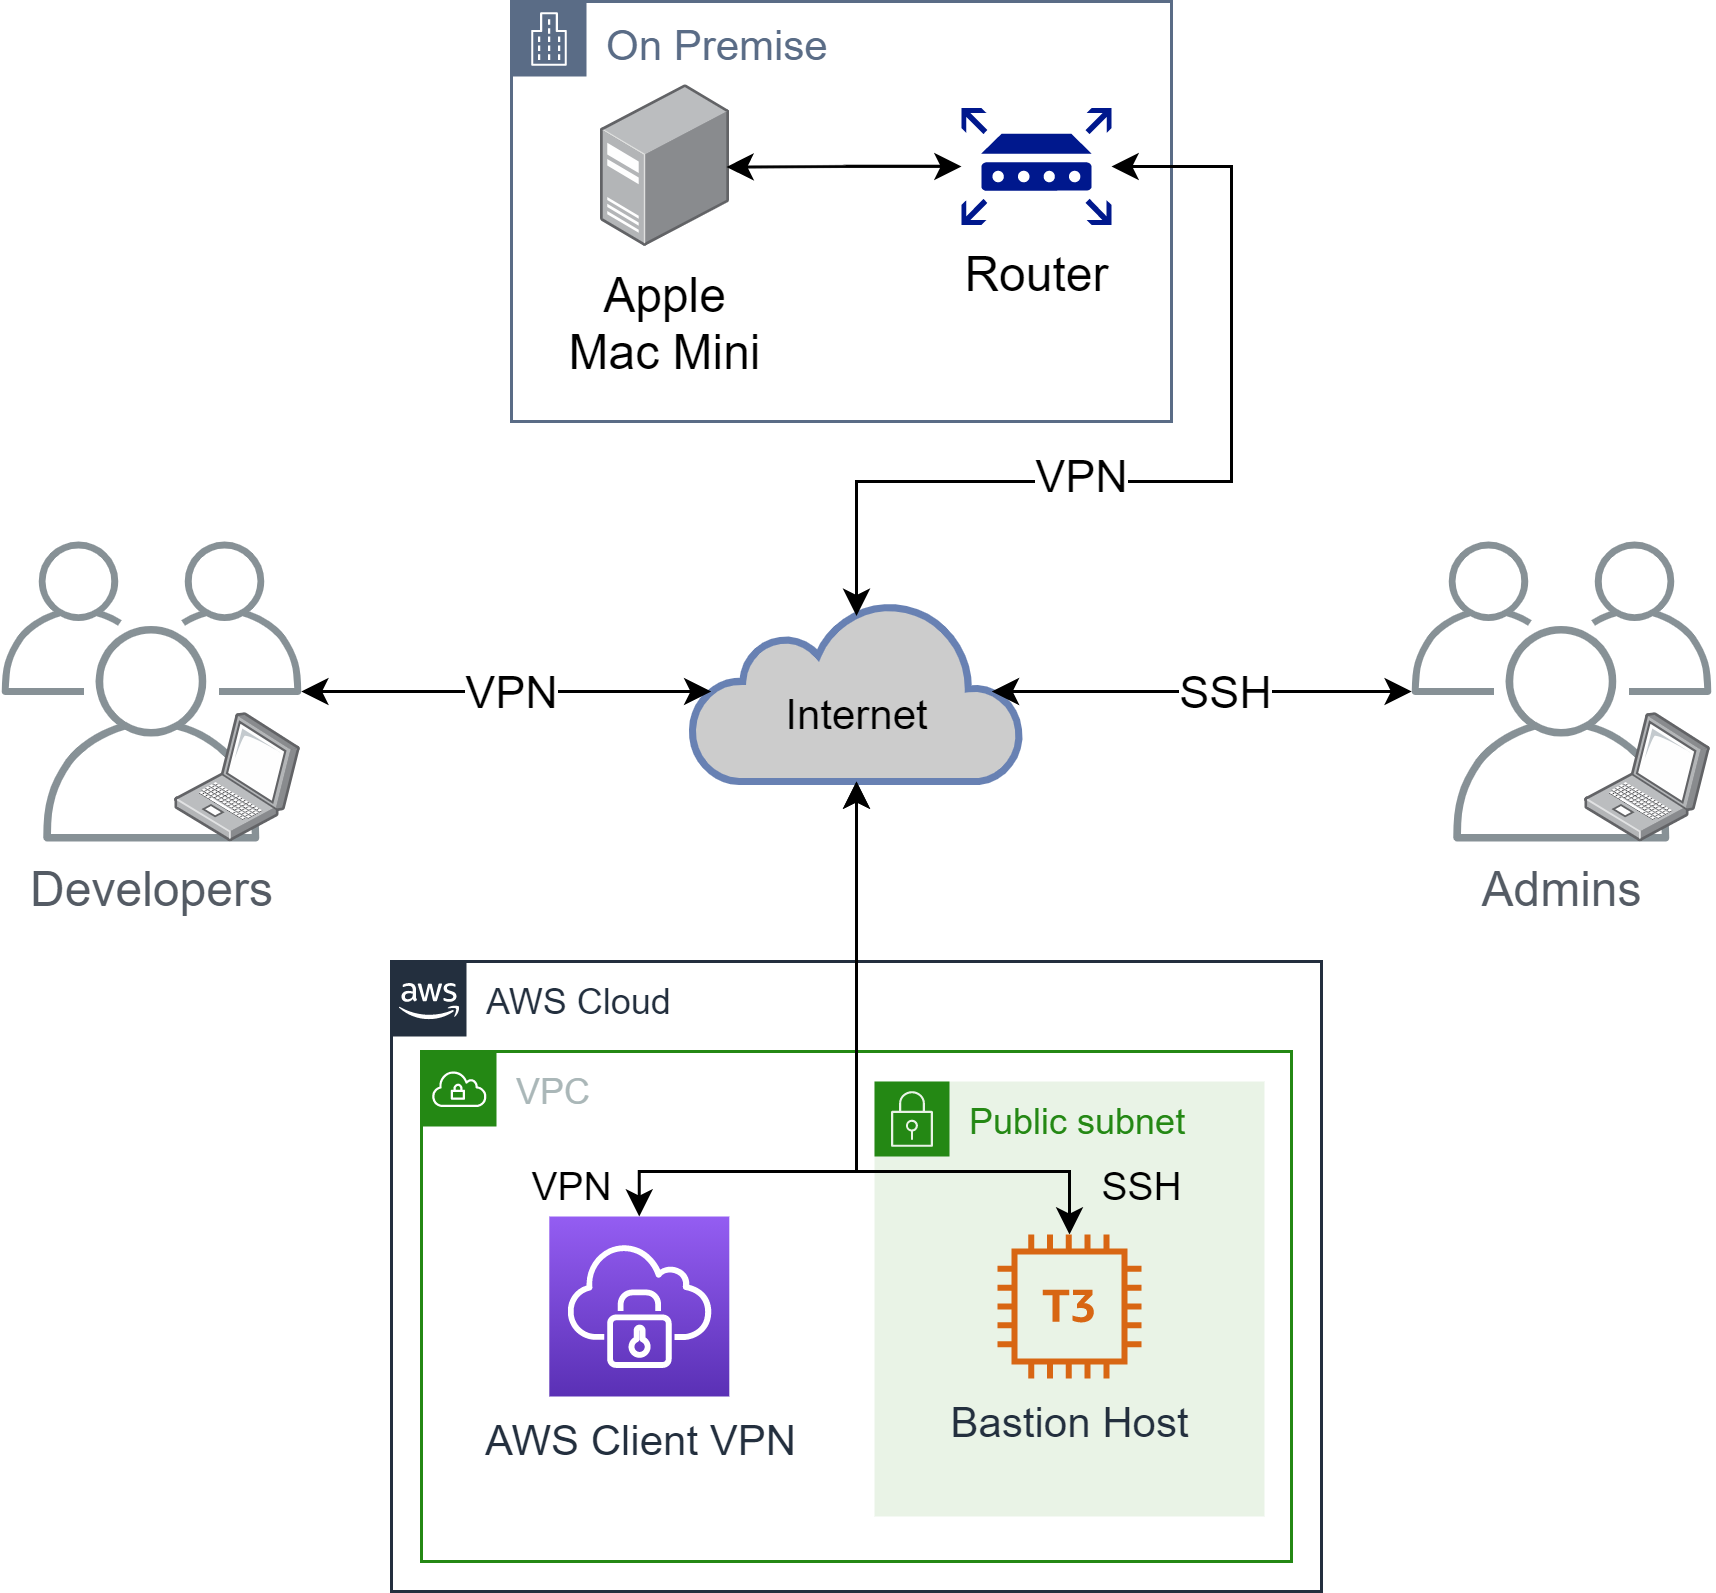
\includegraphics[width=0.9\textwidth]{sphere_devops_arch_part1}
    			\caption{DevOps - Architettura Cloud - Esterna}
    			\label{fig:sphere_devops_arch_part1}
    	    \end{figure}
    	
    	    L'architettura Cloud, descritta negli schemi \ref{fig:sphere_devops_arch_part1} e \ref{fig:sphere_devops_arch_part2}, consiste nel raggruppamento delle risorse in una rete \textbf{AWS VPC} con le seguenti caratteristiche:
    	    \begin{itemize}
    	        \item \textbf{Regione}: Europa Centrale (Francoforte)
    	        \item \textbf{CIDR Block}: \verb|10.0.0.0/16|
    	        \item \textbf{Availability Zone}: \emph{Multi-AZ}
    	        \item \textbf{Subnets}
    	        \begin{itemize}
    	            \item \emph{Public}: \verb|10.0.1.0/24|
    	            \item \emph{Private (EC2)}: \verb|10.0.11.0/24| - \verb|10.0.12.0/24| - \verb|10.0.13.0/24|
    	            \item \emph{Private (ELB)}: \verb|10.0.21.0/24| - \verb|10.0.22.0/24| - \verb|10.0.23.0/24|
    	            \item \emph{Private (RDS)}: \verb|10.0.103.0/24| - \verb|10.0.104.0/24| - \verb|10.0.105.0/24|
    	        \end{itemize}
    	        \item \textbf{NAT Gateway}: singolo per traffico in uscita
    	    \end{itemize}
    	    
    	    \begin{figure}[H]
    			\centering
    			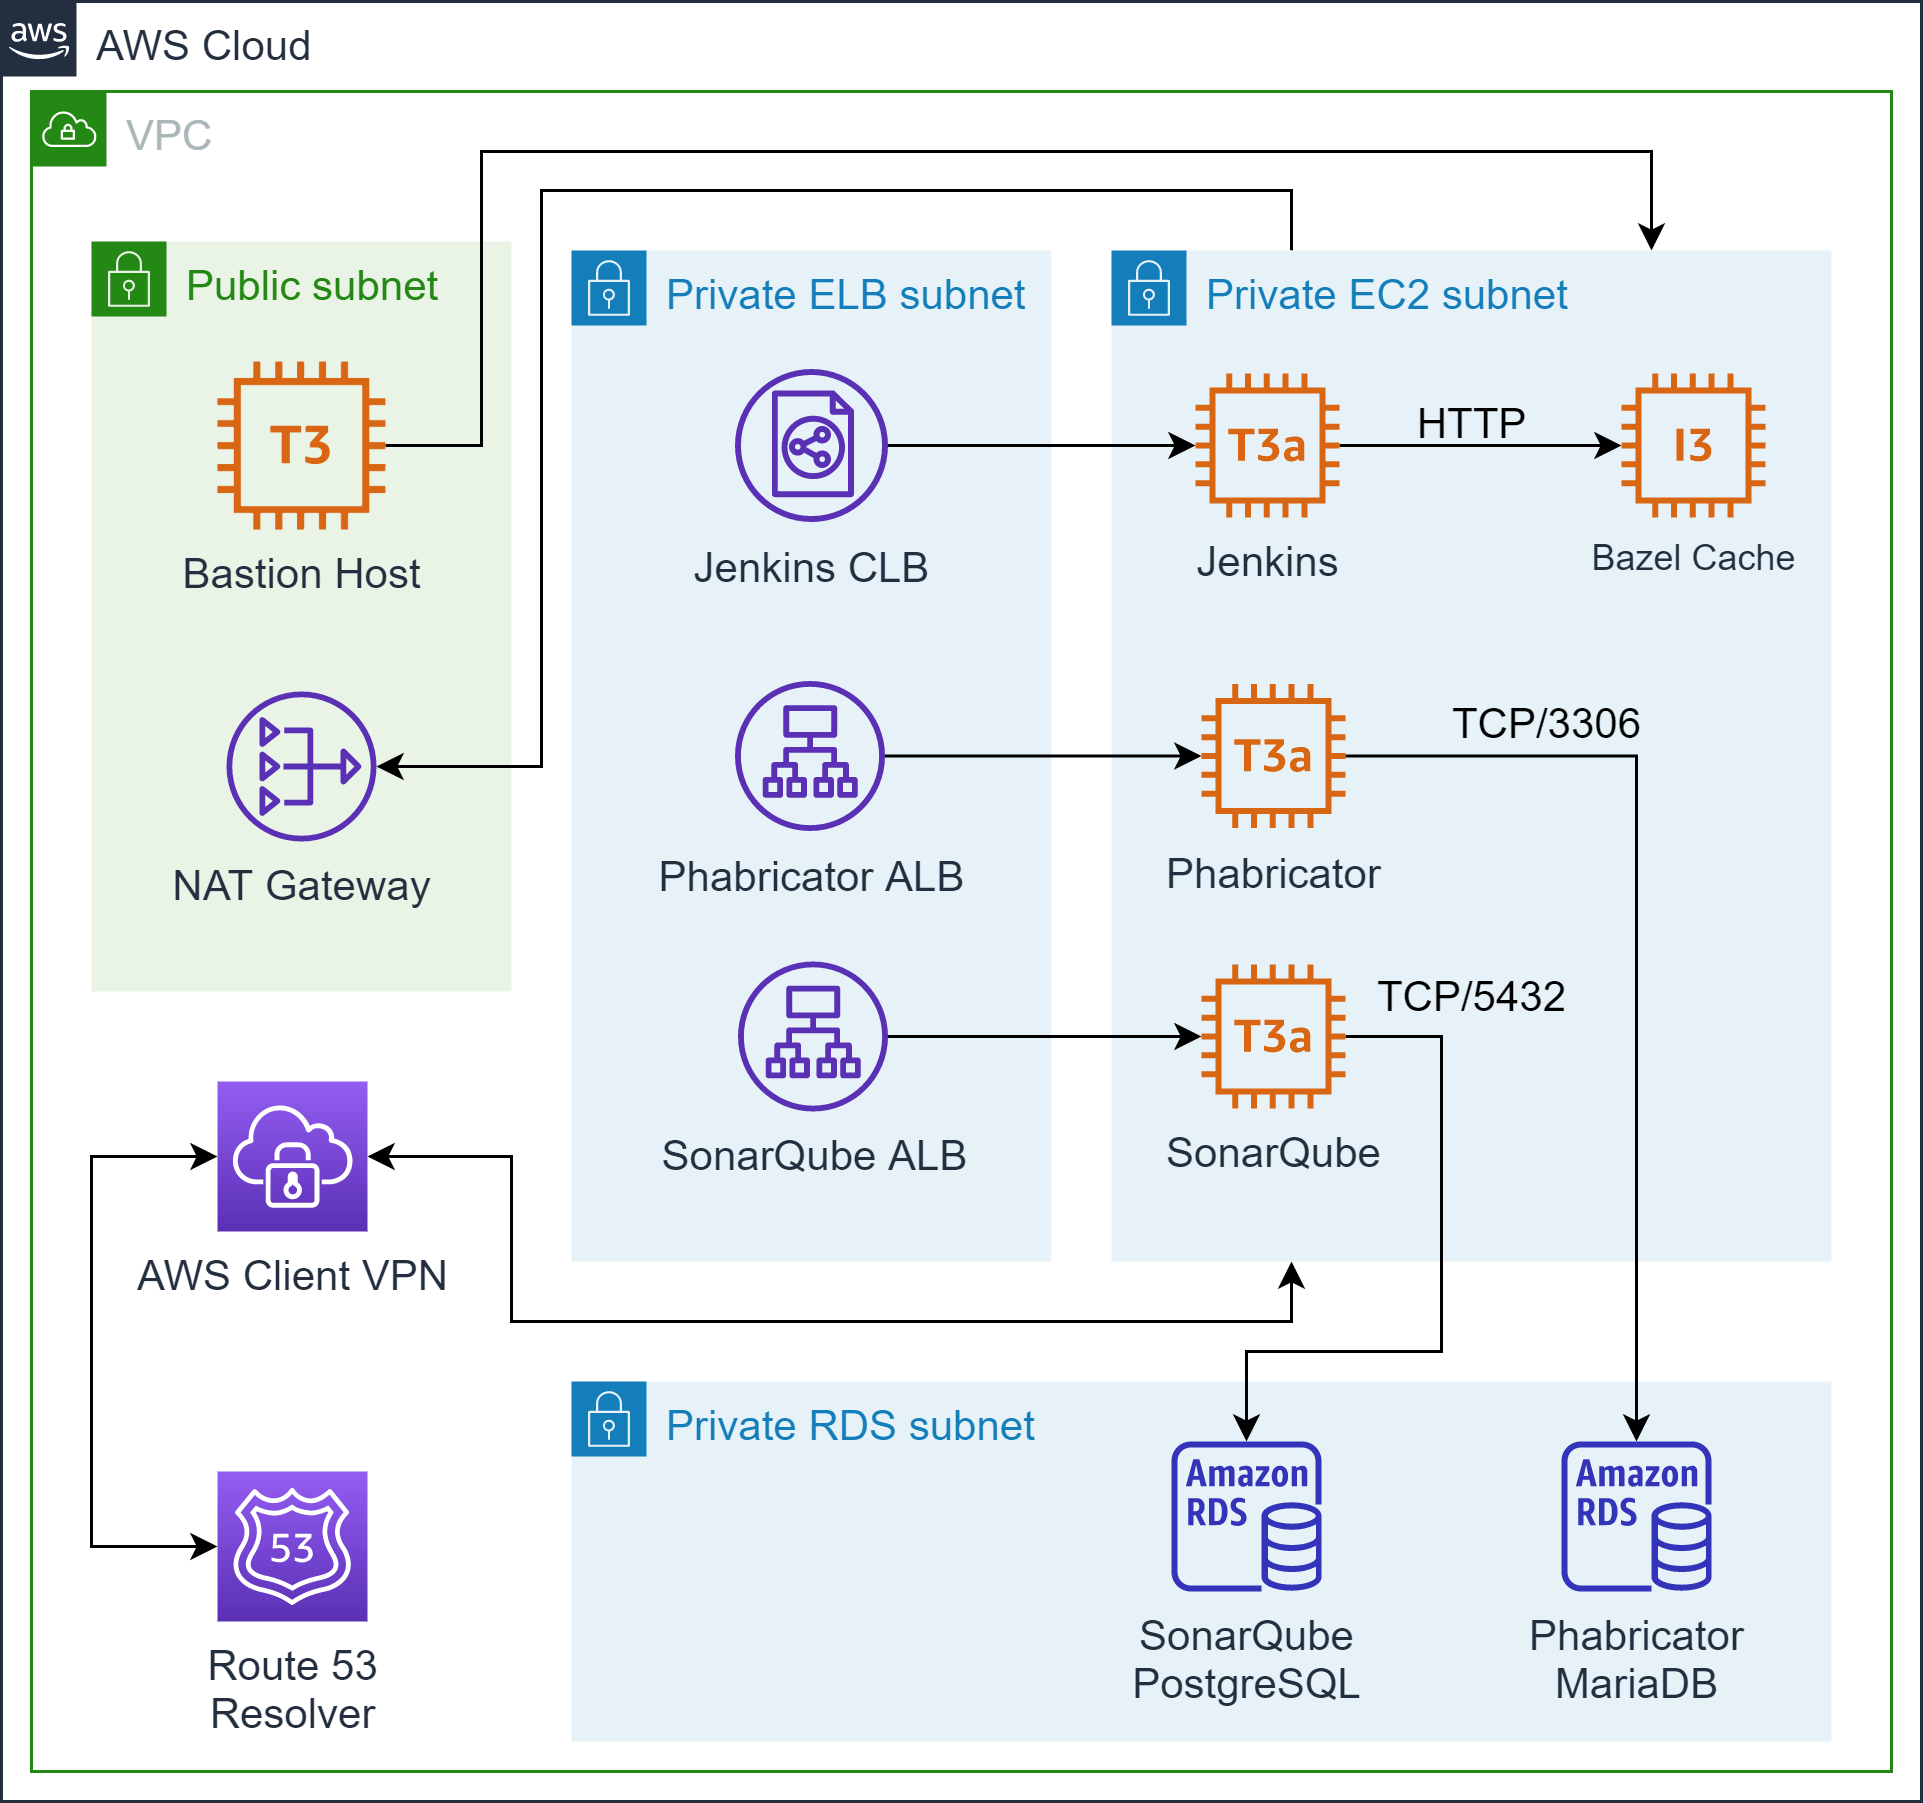
\includegraphics[width=\textwidth]{sphere_devops_arch_part2}
    			\caption{DevOps - Architettura Cloud - Interna}
    			\label{fig:sphere_devops_arch_part2}
    	    \end{figure}
    	
    	    \paragraph{Accesso VPN}
    	    All'interno della VPC è stata creata una istanza di \textbf{AWS Client VPN}, un servizio di Virtual Private Network basato su \emph{OpenVPN} che permette, mediante il rilascio di appositi certificati firmati e l'associazione alle subnet della VPC, l'accesso alle reti private mediante un \emph{tunneling} dedicato. Associando il servizio di VPN con il servizio di DNS privato \textbf{AWS Route 53 Resolver}, si ottiene una navigazione senza intoppi come se fossimo online.
    	    Il servizio è stato configurato per fornire IP della classe \verb|10.1.0.0/16| e agganciarsi mediante una \emph{route table} alle subnet private della VPC come descritte sopra.
    	    
    	    \paragraph{Accesso SSH}
    	    Un paradigma comune nella creazione di infrastrutture cloud è l'utilizzo di una macchina denominata \textbf{Bastion Host}, con IP pubblico (o DNS pubblico) raggiungibile, che funge da "controllore" sempre attivo per gli accessi SSH alle macchine private nella VPC. Utilizzare questo sistema permette di:
    	    \begin{itemize}
    	        \item Mantenere le macchine private sempre al sicuro in una subnet interna;
    	        \item Scremare gli accessi SSH mediante appositi controlli o esclusioni sul Bastion Host;
    	        \item Aprire all'esterno solo la porta SSH con un sistema a 2 step;
    	        \item Il resto del traffico dovrà passare solo dalla VPN precedentemente creata.
    	    \end{itemize}
    	    Nella infrastruttura definita, questa macchina viene creata mediante AWS EC2 con una istanza di tipo \verb|t3.nano| (1 vCore, 1 GiB RAM) e storage EBS GP2 da 8 GiB, nella subnet pubblica (ottiene IP pubblico esterno). Associata a questa macchina si utilizza generalmente anche un DNS o Load Balancer con DNS per facilitare l'accesso, che non verrà descritto in questa architettura.
    	    
    	    \paragraph{Macchine Virtuali}
    	    Ogni strumento verrà installato in una singola istanza \textbf{AWS EC2} di grandezze e risorse differenti in base ai requisiti del singolo applicativo, specificatamente:
    	    \begin{itemize}
    	        \item \textbf{Bazel Cache}: Istanza \verb|i3.large| (Storage Optimized), 2 vCore, 15.25 GiB RAM, 475GB SSD NVMe;
    	        \item \textbf{Phabricator/Jenkins/SonarQube}: Istanza \verb|t3a.medium| (General Purpose), 2 vCore, 4 GiB RAM, Storage EBS GP2.
    	    \end{itemize}
    	    
    	    \paragraph{Database}
    	    Gli strumenti che necessitano connessione ad un database relazionale (Phabricator e SonarQube), sono stati configurati utilizzando istanze \emph{managed} di \textbf{AWS RDS} con il relativo engine di database necessario, in configurazione \emph{Single AZ} e con backup periodici automatici. In particolare troviamo le seguenti configurazioni:
    	    \begin{itemize}
    	        \item \textbf{Phabricator MariaDB}: istanza \verb|db.t3.small| (2 vCore, 2 GiB RAM), engine \emph{MariaDB} 10.3.23, 20 GiB storage con autoscaling fino a 50 GiB;
    	        \item \textbf{SonarQube PostgreSQL}: istanza \verb|db.t3.micro| (2 vCore, 1 GiB RAM), engine \emph{PostgreSQL} 12.4, 20 GiB storage con autoscaling fino a 50 GiB.
    	    \end{itemize}
    	
    	\pagebreak
    	
    	\section{Creazione Infrastruttura}
    	    
    	    \subsection{Struttura \emph{IaC}}
    	
        	    L'infrastruttura è stata definita mediante l'uso di \textbf{Terraform} \verb|0.14|, provider AWS \verb|< 3.15| (a causa di un bug in versioni superiori riguardo l'utilizzo dell'ACL su Bucket S3, necessario all'uso del modulo di Bastion Host scelto). Il progetto ha la seguente struttura, creata per suddividere gli ambienti di deployment rispetto ai moduli riusabili:\\
                \begin{forest}
                  for tree={
                    font=\ttfamily,
                    grow'=0,
                    child anchor=west,
                    parent anchor=south,
                    anchor=west,
                    calign=first,
                    inner xsep=7pt,
                    edge path={
                      \noexpand\path [draw, \forestoption{edge}]
                      (!u.south west) +(7.5pt,0) |- (.child anchor) pic {folder} \forestoption{edge label};
                    },
                    before typesetting nodes={
                      if n=1
                        {insert before={[,phantom]}}
                        {}
                    },
                    fit=band,
                    before computing xy={l=15pt},
                  }  
                [devops\_iac
                  [environments
                    [tools
                        [bazel\_cache]
                        [jenkins]
                        [phabricator]
                        [sonarqube]
                    ]
                  ]
                  [modules
                    [alb]
                    [client\_vpn]
                    [dns\_cert]
                    [ec2]
                    [elb]
                    [rds]
                    [vpc]
                  ]
                ]
                \end{forest}
        	    
        	    \paragraph{Inizializzazione}
        	    Terraform è stato inizializzato con la seguente configurazione, che permette di utilizzare un \emph{Bucket S3} come storage remoto del suo stato, abilitando l'utilizzo da parte di più sviluppatori:
        	    \begin{lstlisting}
terraform {
    required_version = ">= 0.14.0"

    required_providers {
        aws = "< 3.15"
    }

    backend "s3" {
        bucket     = "perceptolab-devops"
        region     = "eu-central-1"
    }
}
        	    \end{lstlisting}
        	    
        	    \paragraph{Moduli}
        	    Ogni modulo contenuto in \verb|modules| segue una struttura di divisione delle risorse, dalle variabili in input e variabili in output, come da \emph{Best Practice} su Terraform:
        	    \begin{itemize}
        	        \item \textbf{main.tf}: contiene tutte le risorse create dal modulo parametrizzate sulle variabili in ingresso e le fonti dati (\emph{queried-only});
        	        \item \textbf{variables.tf}: variabili in ingresso del modulo, permettono di riutilizzare il modulo generalizzando la sua implementazione;
        	        \item \textbf{output.tf}: variabili in uscita dal modulo, recuperate dalle varie risorse create dallo stesso e rielaborate per riutilizzo da parte di altre risorse o moduli richiamanti.
        	    \end{itemize}
        	    
        	    Prendendo come esempio il modulo di creazione di una generica macchina virtuale \emph{EC2} possiamo trovare la seguente struttura nel suo file \verb|main.tf|:
        	    \begin{lstlisting}
# Searches for the latest Amazon Linux 2 AMI
data "aws_ami" "amazon-linux-2" {
  most_recent = true
  (...)
}

resource "aws_instance" "ec2_instance" {
  # Which Amazon Machine Image to use as base root device
  ami = var.ami != "" ? var.ami : data.aws_ami.amazon-linux-2.id

  key_name      = var.key_name # SSH Key Name
  instance_type = var.instance_type # EC2 Instance Type
  (...)
  dynamic "ephemeral_block_device" {
    for_each = var.ephemeral_volumes # Configure EC2 Ephemeral Volumes if available

    content {
      virtual_name = ephemeral_block_device.key
      device_name  = ephemeral_block_device.value
    }
  }
  (...)
}
        	    \end{lstlisting}
        	    
        	    Le variabili richiamate mediante la sintassi \verb|var.<name>| sono definite nel file \\\verb|variables.tf| in base al loro nome, tipo (stringa, numero, booleano, key-value, lista), descrizione e valore di default se applicabile:
        	    \begin{lstlisting}
variable "volume_size" {
  type        = number
  default     = 9
  description = "EBS Root FS volume size in GiB"
}

variable "ephemeral_volumes" {
  type        = map(string)
  default     = {}
  description = "AWS EC2 Instance Store ephemeral devices"
}
        	    \end{lstlisting}
        	    
        	    Mentre tutte le variabili di output risultanti dalla creazione delle risorse sopra definite vengono dichiarate all'interno del file \verb|output.tf| seguendo la reference dell'oggetto creato dalla \emph{resource} definita precedentemente:
        	    \begin{lstlisting}
output "id" {
  value = aws_instance.ec2_instance.id
}

output "private_ip" {
  value = aws_instance.ec2_instance.private_ip
}
        	    \end{lstlisting}
        	
            	\paragraph{Environment}
            	I moduli così creati con Terraform così inizializzato, permettono di essere composti in ciò che vengono definiti gli \textbf{ambienti}, ovvero set di moduli sia locali che remoti (mediante \emph{Terraform Registry}) che definiscono un intero deployment. In questo progetto vi è un solo ambiente definito da diversi sotto-ambienti che definiscono a loro volta i singoli deployment per i singoli strumenti utilizzati, vi sarà quindi un \verb|main.tf| generale dell'ambiente che definisce i sotto-ambienti da utilizzare:
            	\begin{lstlisting}
# Define VPC module
module "vpc" {
  source = "../../modules/vpc"
  vpc_cidr_block = "10.0.0.0/16"
}

# Define Bastion Host via Terraform Registry
module "bastion-host" {
  source  = "Guimove/bastion/aws"
  (...)
}

# Defines SonarQube sub environment
module "sonarqube" {
  source = "./sonarqube"
  (...)
}
            	\end{lstlisting}
    	
    	    \subsection{Struttura \emph{CaC}}
    	    
    	        I vari strumenti sono stati configurati utilizzando \textbf{Ansible} \verb|2.9.x|, e l'integrazione da parte del plugin di \textbf{ansible.posix} in versione \verb|1.1.1| e di \textbf{community.general} in versione \verb|1.1.0|, entrambi gestiti mediante \emph{Ansible Galaxy}, un tool accessorio ad Ansible stesso che permette di gestire le dipendenze e i plugin all'interno dei ruoli e playbook definiti. Il progetto, contenuto nello stesso repository, ha la seguente struttura:\\
    	        \begin{forest}
                  for tree={
                    font=\ttfamily,
                    grow'=0,
                    child anchor=west,
                    parent anchor=south,
                    anchor=west,
                    calign=first,
                    inner xsep=7pt,
                    edge path={
                      \noexpand\path [draw, \forestoption{edge}]
                      (!u.south west) +(7.5pt,0) |- (.child anchor) pic {folder} \forestoption{edge label};
                    },
                    before typesetting nodes={
                      if n=1
                        {insert before={[,phantom]}}
                        {}
                    },
                    fit=band,
                    before computing xy={l=15pt},
                  }  
                [devops\_iac
                  [ansible
                    [inventory]
                    [roles
                        [base-docker]
                        [bazel-cache-service
                            [tasks]
                            [templates]
                        ]
                        [jenkins-service]
                        [phabricator-service]
                        [sonarqube-service]
                    ]
                  ]
                ]
                \end{forest}
                
                \paragraph{Inventory}
                Utilizzando una cloud platform, non possiamo sapere a priori l'indirizzo IP privato del server target ne l'indirizzo IP esterno del Bastion Host, motivo per cui al posto di utilizzare un \emph{inventory} statico, utilizziamo un \textbf{\emph{dynamic inventory}}, formato da uno \textbf{script Python} \verb|ec2.py| ed un file di configurazione \verb|ec2.ini| forniti dai creatori di Ansible. Questo script sarà avviato da Ansible ed effettuerà delle query sulle risorse cloud, creando un \emph{inventory} utilizzabile dal runtime del tool stesso.
                
                \paragraph{Configurazione e Dipendenze}
                Nella sottocartella \verb|ansible|, oltre alla struttura descritta, vi sono dei file che definiscono la configurazione di Ansible stesso e le dipendenze dei nostri \emph{playbook}. Tali file sono nominati \verb|ansible.cfg| e \verb|requirements.yml|, il primo definito con una singola modifica:
                \begin{lstlisting}[language={Ini}]
[defaults]
# Host key checking is enabled by default
host_key_checking = False
                \end{lstlisting}
                mentre il secondo presenta la seguente struttura, indicando le dipendenze relative ad \emph{Ansible Galaxy}:
                \begin{lstlisting}[language=yaml]
---
collections:
  - name: ansible.posix
    version: 1.1.1
  - name: community.general
    version: 1.1.0
                \end{lstlisting}
                
                \paragraph{Playbooks}
                Sempre nella sottocartella \verb|ansible|, sono stati inseriti dei file YAML che definiscono i \emph{playbooks} più esterni e quindi più specifici, al cui interno vengono utilizzati i \emph{roles} definiti dalle cartelle create. Questi \emph{playbooks} definiscono il nome dell'host target, le variabili in ingresso dall'esterno (al momento del richiamo di Ansible da terminale) e i ruoli da installare su quel target host. Prendendo la configurazione di SonarQube come esempio, possiamo notare come il nome dell'host sia derivato dal \textbf{tag} della macchina \textbf{EC2} creata precedentemente:
                \begin{lstlisting}[language=yaml]
---
- name: SonarQube server setup
  hosts: tag_Name_pl_tools_sonarqube_ec2
  become: yes
  gather_facts: no
  vars:
    ansible_ssh_common_args: -o ProxyCommand="ssh -W %h:%p -i sshkey.pem ec2-user@{{ bastion }}"
    postgres_host: "{{ postgres_host }}"
    postgres_user: "{{ postgres_user }}"
    postgres_pwd: "{{ postgres_pwd }}"
  roles:
    - base-docker
    - sonarqube-service
                \end{lstlisting}
                
                \paragraph{Templating}
                All'interno di ogni ruolo, ove necessario, sono presenti 2 sottocartelle, una contenente i \emph{playbooks} che definiscono quel ruolo (\verb|tasks|) e una seconda chiamata \verb|templates| contenente eventuali file da copiare sulla macchina target che possono avere formato \verb|j2|, ovvero che utilizzano il template engine integrato in Ansible chiamato \textbf{Jinja2}. Mediante questo engine è possibile sostituire all'interno dei file template i valori di determinati placeholder, ad esempio a partire dalle variabili in ingresso al \emph{playbook} oppure a valori creati durante l'esecuzione (ad esempio password autogenerate).
    	
    	\section{Configurazione di Bazel Cache}
    	
    	    L'utilizzo della cache remota in Bazel ci permette di velocizzare notevolmente le build effettuate consecutivamente, dove i cambiamenti incrementali sono piccoli in comparazione alla grandezza della codebase completa. La cache si presenta come un semplice \textbf{HTTP Server} con relativo storage, nel nostro caso il deployment è composto da:
    	    \begin{enumerate}
    	        \item \textbf{NGINX con WebDAV}: fornisce una interfaccia HTTP Plain con cui interagire con la cache su disco, mediante richieste HTTP \emph{GET} e \emph{PUT} gestite da Bazel stesso;
    	        \item \textbf{Cache Cleaner}: \emph{cron job} giornaliero che cancella i file più vecchi di 2 settimane (14 giorni) all'interno della cache su disco;
    	        \item \textbf{Instance Storage}: la macchina EC2 scelta fornisce un disco SSD NVMe da 475 GiB utilizzato come storage "effimero", ovvero che viene eliminato ad ogni riavvio della macchina stessa, ma che offre performance estremamente elevate e consistenti. Sia NGINX che il Cleaner hanno accesso in R/W a tale storage.
    	    \end{enumerate}
    	    
    	    \paragraph{NGINX}
    	    L'istanza di NGINX viene installata mediante l'uso di un \textbf{container Docker}, immagine basata su \verb|ubuntu:focal| mediante il quale viene installato il server e configurato per ascoltare su porta \verb|80| e path \verb|/cache|:
    	    \begin{lstlisting}[language=docker]
FROM ubuntu:focal
RUN apt-get update && \
    DEBIAN_FRONTEND=noninteractive apt-get install -y --no-install-recommends nginx nginx-extras apache2-utils
# (...)
CMD nginx -g "daemon off;"
    	    \end{lstlisting}
    	    
    	    \paragraph{Cleaner}
    	    Anche il \emph{Cache Cleaner} viene installato mediante creazione di una immagine e relativo \textbf{container Docker}, basato su \verb|alpine:3| dove viene semplicemente avviato il demone \verb|crond| con il relativo cronjob configurato:
    	    \begin{lstlisting}[language=docker]
FROM alpine:3
# (...)
COPY cronjobs /etc/crontabs/root
CMD ["crond", "-f", "-d", "8"]
    	    \end{lstlisting}
    	    
    	    \paragraph{Storage}
    	    Per configurare ed utilizzare l'\emph{Instance Storage} su una macchina EC2, si necessita di effettuare un \emph{format} del volume, un \emph{mount} su un determinato percorso (nel nostro caso \verb|/mnt/bazel_cache/cache|) e di fornire i permessi necessari ai container creati mediante Docker:
    	    \begin{lstlisting}[language=yaml]
(...)
- name: Create a ext4 filesystem on ephemeral storage
  become: yes
  community.general.filesystem:
    dev: /dev/nvme0n1
    fstype: ext4
    
- name: Mount ephemeral storage
  become: yes
  ansible.posix.mount:
    src: /dev/nvme0n1
    path: /mnt
    fstype: ext4
    opts: rw,noatime
    state: mounted
(...)
    	    \end{lstlisting}
    	    
    	    La creazione delle 2 immagini citate (NGINX, Cleaner), l'istanziamento dei relativi container mediante Docker, e la configurazione dell'instance storage sono stati effettuati mediante l'utilizzo di un \emph{role} dedicato con \textbf{Ansible}. A corredo della configurazione del server in se, viene creata anche una \textbf{entry nel DNS privato} che permette di accedere alla cache per le macchine interne alla VPC senza conoscerne l'IP privato.
    	
    	\section{Configurazione di Phabricator}
    	
    	    Il deployment di Phabricator consiste in 2 componenti separate: il \textbf{Database} e l'istanza in se mantenuta sulla macchina virtuale EC2 creata. Usando Ansible definiamo un \emph{playbook} composto da 2 parti:
    	    \begin{enumerate}
    	        \item \textbf{Environment}: effettua il setup del database gestendolo direttamente dalla macchina EC2 di Phabricator stesso, essendo l'istanza di RDS privata nella VPC. Crea l'utenza di Phabricator e da i permessi corretti per creare e gestire il proprio schema all'interno di MariaDB, effettua inoltre il setup dei file di configurazione di Phabricator localmente sulla macchina;
    	        \item \textbf{Instance}: mediante l'utilizzo di Docker e l'immagine pubblica \\\verb|phabricator/phabricator:stable|, crea un container a cui aggancia i file di configurazione ed un volume locale per mantenere i dati sulla macchina. Dopo la creazione, effettua il setup del database pilotando direttamente l'istanza creata di Phabricator usando una \emph{shell} tramite Docker.
    	    \end{enumerate}
    	
    	    \paragraph{Database}
    	    L'istanza di RDS basata su MariaDB viene configurata per creare una utenza con i permessi necessari ad effettuare le operazioni di cui necessita Phabricator. In particolare Ansible fornisce una azione chiamata \verb|mysql_user| che permette di creare, modificare e cancellare utenze in un database \emph{MySQL-based} (come MariaDB):
    	    \begin{lstlisting}[language=yaml]
- name: Create Phabricator MariaDB user
  become: yes
  become_user: ec2-user
  mysql_user:
    name: "phabricator"
    host: "%"
    password: "{{ lookup('password', 'phabricator/.passwd length=32 chars=ascii_letters,digits,hexdigits') }}"
    priv: "phabricator_%.*:<list of all permissions>"
    (...)
    	    \end{lstlisting}
    	    
    	    \paragraph{Configurazione}
    	    Phabricator necessita di un file \verb|local.json| dove mantiene le configurazioni statiche, creato sostituendo i valori necessari dati in ingresso al \emph{playbook} mediante il sistema di templating di Ansible, le cui configurazioni salienti sono le seguenti:
    	    \begin{itemize}
    	        \item \verb|security.require-https|: forza l'utilizzo di HTTPS (\emph{TLS Termination} su AWS ALB);
    	        \item \verb|auth.email-domains|: abilita l'iscrizione solo da email dei domini permessi;
    	        \item \verb|cluster.mailers|: configurazione del sistema di mailing interno per le notifiche;
    	        \item \verb|mysql.<var>|: configurazione del database associato all'istanza;
    	        \item \verb|recaptcha.<var>|: configurazione di \emph{reCAPTCHA} per evitare accessi fraudolenti da parte di bot.
    	    \end{itemize}
    	
    	\section{Configurazione di Jenkins}
    	
    	    Il deployment di Jenkins si compone di una singola macchina dove l'istanza gestirà tutti dati necessari utilizzando lo storage integrato con AWS EBS, in cui mediante Ansible viene creato un container basato sull'immagine \\\verb|jenkinsci/blueocean:1.24.4| configurando l'ambiente nel seguente modo:
    	    \begin{enumerate}
    	        \item \textbf{Volumi}: per mantenere i dati del container sullo storage della macchine, viene creato un \emph{Docker Volume} gestito e montato nel container sul path \verb|/var/jenkins_home|;
    	        \item \textbf{Container}: il container di Jenkins Blue Ocean viene creato esponendo le porte \verb|80| e \verb|50000|, utilizzate rispettivamente per l'accesso alla Web UI e la connessione di \emph{Agent} esterni mediante protocollo \emph{JNLP};
    	        \item \textbf{Plugins}: a seguito della creazione del container vengono installati i plugins definiti in un file \verb|plugins.txt|, che lista gli ID dei plugins come definiti nel repository di Jenkins;
    	        \item \textbf{Arcanist}: per permettere a Jenkins di applicare le patch provenienti da Pull Request su Phabricator, viene installato il runtime PHP assieme alla libreria di \emph{libphutil} e la CLI di \emph{Arcanist} direttamente nel container.
    	    \end{enumerate}
    	    
    	    \paragraph{Arcanist}
    	    L'installazione di Arcanist all'interno del container avviene mediante l'utilizzo di \verb|docker exec|, un comando di Docker che permette di avviare comandi utilizzando una shell interna ad un container. In questo caso verrà installato \emph{PHP 7} dai repository di \textbf{Alpine Linux} (sistema su cui è basato l'immagine usata) e sia \emph{libphutil} che \emph{Arcanist} verranno installati clonando i rispettivi repository da Github:
    	    \begin{lstlisting}[language=yaml]
- name: Install PHP for Arcanist
  become: yes
  become_user: ec2-user
  command: "docker exec -it -u 0 jenkins apk add --no-cache --update-cache php7 php7-curl php7-json"
(...)
- name: Clone Arcanist
  become: yes
  become_user: ec2-user
  ignore_errors: yes
  command: "docker exec -it jenkins git clone https://github.com/phacility/arcanist.git /var/jenkins_home/arcanist"
    	    \end{lstlisting}
    	
        	\subsection{Agent su AWS EC2}
        	
        	    Per gestire degli \emph{Agent} utilizzando macchine virtuali AWS EC2, è necessario installare su Jenkins il rispettivo \textbf{plugin} che una volta configurato permette di gestire un \textbf{pool di server} in modo da mantenere le risorse disponibili quando necessario e di ridurre i costi se non ci si aspetta traffico sulla piattaforma. Il plugin si interfaccia con AWS mediante un \textbf{IAM Role} configurato ad-hoc per poter accedere alle API della piattaforma EC2 e creare così sia istanze \emph{on demand} che di tipo \emph{spot} per risparmiare sui costi dove possibile. Le macchine gestite da Jenkins vengono inoltre \textbf{distrutte quando non utilizzate}, permettendo un grado di cost saving consistente, specialmente in giorni non lavorativi.\\*
        	    
        	    La macchina che verrà creata dal plugin utilizzando come immagine di partenza un \textbf{AMI} (\emph{Amazon Machine Image}) creato in precedenza, con al suo interno le seguenti dipendenze:
        	    \begin{itemize}
        	        \item OpenJDK 11
        	        \item Git con LFS
        	        \item Arcanist (con \emph{PHP 7} e \emph{libphutil})
        	        \item Docker (per uso ambiente di build)
        	        \item Sonar Scanner (per analisi con \emph{SonarQube})
        	    \end{itemize}
        	    
        	    Jenkins, una volta creata la macchina mediante l'utilizzo del plugin EC2, accederà ad essa sfruttando \textbf{SSH} (nella stessa rete privata) e la comanderà come se fosse un semplice host linux remoto, permettendo di avviare comandi remoti, accedere ai suoi file e quindi implementare l'intera pipeline definita. Il \textbf{tipo di istanza} scelta per effettuare build dei servizi di backend è di tipo \verb|c5a.2xlarge| con 8 vCore e 16 GiB di RAM.
        	
        	\subsection{Agent macOS On-Premise}
    	
    	        Per effettuare compilazioni di artefatti, librerie e dipendenze per \textbf{Apple iOS} (OS mobile), è necessario utilizzare un ambiente basato su \textbf{macOS}, in questo caso un \textbf{Apple Mac Mini} gestito \emph{on-premise} con installato l'ultimo aggiornamento di \emph{macOS Big Sur} ed \verb|XCode 12.4| che offre supporto ad \verb|iOS 14.4|.\\*
    	        
    	        Sul Mac viene così configurato un \textbf{Jenkins Agent JNLP}, sfruttando la connessione VPN instaurata dal router \emph{on-premise} verso la rete di AWS, non prima di aver effettuato il setup dell'ambiente installando le seguenti dipendenze:
    	        \begin{itemize}
    	            \item OpenJDK 8 (o 11)
    	            \item Git con LFS
    	            \item Arcanist (con \emph{PHP 7} e \emph{libphutil})
    	            \item Bazel 3.7
    	            \item Eventuali altre dipendenze del sistema operativo (es. XCode Build Tools)
    	        \end{itemize}
    	        
    	        Da Jenkins verrà configurato l'agent, che genererà un file \verb|agent.jar| ed una chiave di autenticazione univoca, entrambi da riportare localmente sulla macchina Mac. L'agent viene avviato mediante uno \emph{script bash} installato come servizio di sistema all'avvio (mediante \verb|launchctl|) con la seguente sintassi:
    	        \begin{lstlisting}[language=bash]
#!/bin/bash -l
/usr/bin/java -Xms256m -Xmx2048m -jar /Users/jenkins/Documents/scripts/agent.jar -jnlpUrl "https://jenkins.domain.com/computer/macos/slave-agent.jnlp" -secret "<secret>" -workDir "/Users/jenkins/build/"
    	        \end{lstlisting}
    	
    	\section{Configurazione di SonarQube}
    	
    	    Il deployment di SonarQube, come per Phabricator, si compone di una macchina virtuale EC2 e di un database relazionale. Mediante l'utilizzo di Ansible vengono effettuate le operazioni di configurazione dell'ambiente e di deployment del servizio in se, con il seguente schema operativo:
    	    \begin{itemize}
    	        \item \textbf{Database}: viene creato il database e l'utenza che userà SonarQube, a cui vengono dati i permessi di \verb|CONNECT/CREATE| ed una password autogenerata in fase di creazione;
    	        \item \textbf{Environment}: nonostante Sonar utilizzi un DB relazionale esterno, internamente sfrutta una istanza di \emph{ElasticSearch} che necessita di configurazioni aggiuntive nell'ambiente in cui viene creato. In particolare vengono modificate le seguenti variabili di sistema:
    	        \begin{itemize}
    	            \item \verb|vm.max_map_count|: numero massimo di aree di mapping di memoria che un processo può allocare;
    	            \item \verb|fs.file-max|: numero massimo di \emph{file descriptors} aperti nel sistema;
    	            \item \verb|ulimit nproc|: numero massimo di processi aperti per singolo utente;
    	        \end{itemize}
    	        \item \textbf{Deployment}: mediante l'utilizzo di Docker e l'immagine pubblica \verb|sonarqube:lts|, viene creato un container collegato a 4 volumi dedicati a configurazioni, dati, estensioni e file di log. La configurazione del database creato viene passata come \emph{variabili d'ambiente} nel container creato;
    	        \item \textbf{Plugins}: per supportare l'analisi di codice C++ nella versione \emph{Community}, SonarQube necessita di 2 plugin esterni sotto forma di file \verb|.jar|. Tali file vengono copiati all'interno del volume di estensioni creato precedentemente, così da permettere al server di rilevarli ed utilizzarli successivamente.
    	    \end{itemize}
    	    
    	    \paragraph{Database}
    	    L'istanza RDS basata su engine PostgreSQL \verb|12.4| viene configurata per creare una utenza che permetta connessione e creazione di schema, tabelle e quanto necessario a SonarQube stesso, in particolare l'utente \verb|sonarqube| presenta la seguente azione nel \emph{playbook}:
    	    \begin{lstlisting}[language=yaml]
- name: Create SonarQube PostgreSQL user
  become: yes
  become_user: ec2-user
  postgresql_user:
    db: sonarqube
    name: sonarqube
    password: "{{ lookup('password', 'sonarqube/.passwd length=32 chars=ascii_letters,digits,hexdigits') }}"
    priv: "CONNECT/CREATE"
    login_host: "{{ postgres_host }}"
(...)
    	    \end{lstlisting}
    	
    	    \paragraph{Environment}
    	    Per effettuare il setup delle variabili di sistema riguardo limiti di memoria, files e processi, viene sfruttato sia \verb|sysctl| che \verb|ulimit| in base alla variabile da modificare:
    	    \begin{lstlisting}[language=yaml]
(...)
- name: Setup current session sysctl values - file-max
  become: yes
  command: sysctl -w fs.file-max=131072

- name: Setup current session ulimit values - file
  become: yes
  pam_limits:
    domain: ec2-user
    limit_type: '-'
    limit_item: nofile
    value: 131072
(...)
    	    \end{lstlisting}

    	\section{Creazione ambiente di build con Docker}
    	\label{sec:cloud_arch_docker}
    	
    	    Per effettuare compilazioni e renderle sempre riproducibili, indipendentemente dall'ambiente circostante come macchine locali degli sviluppatori o macchine remote per la \emph{CI/CD}, viene creata una \textbf{Immagine Docker} contenente un ambiente controllato e sempre aggiornato sulle esigenze del progetto, che permetta di ottenere tutte le dipendenze in un singolo pacchetto e di evitare variabili inaspettate.\\*
    	    
    	    Tale immagine è basata su \verb|debian:buster-slim| e durante la sua creazione vengono installate le seguenti dipendenze, utili alla compilazione e testing dei servizi di backend e mobile basati su linguaggi C++, Python e in parte Swift:
            \begin{enumerate}
                \item \textbf{C++}: LLVM con Clang e Clang-Tidy
                \item \textbf{Python}: versione \verb|3.7|
                \item \textbf{Bazel}: versione \verb|3.7|
                \item \textbf{Swift}: versione \verb|5.3|, compilata per build su macchine \emph{linux}
                \item \textbf{JDK}: OpenJDK 11, per utilizzo con Bazel per \emph{Code Coverage}
            \end{enumerate}

            L'utilizzo locale di questa immagine viene semplificato mediante l'integrazione di uno \textbf{shell script} che automatizza le build mediante Bazel e permette ad Arcanist di effettuare l'analisi del \emph{linting} ed avviare gli \emph{unit tests} prima di creare una Pull Request su Phabricator. Nelle pipeline di CI/CD viene invece sfruttata l'immagine direttamente da Jenkins mediante il \textbf{Docker Plugin}, creando così un ambiente pronto all'uso ad ogni avvio del processo stesso, che viene eliminato alla sua conclusione.
            
\end{document}